\documentclass{report}
\usepackage{graphicx}
\usepackage{pgfplots}
\begin{document}
\begin{titlepage}
\centering
{\bfseries\LARGE Instituto Tecnol\'ogico de Costa Rica \par}
\vspace{1cm}
{\scshape\Large Facultad de Ingenier\'ia en Computaci\'on \par}
\vspace{3cm}
{\scshape\Huge Simulaci\'on de propagaci\'on \\
de CODEVID-19\par}
\vspace{3cm}
{\itshape\Large Proyecto 2\par}
\vfill
{\Large Emanuelle Jim\'enez S.\par}
{\Large Fabrizio Alvarado B.\par}
\vfill
{\Large Junio 2020 \par}
\end{titlepage}
\newpage
\section{Gr\'afico}
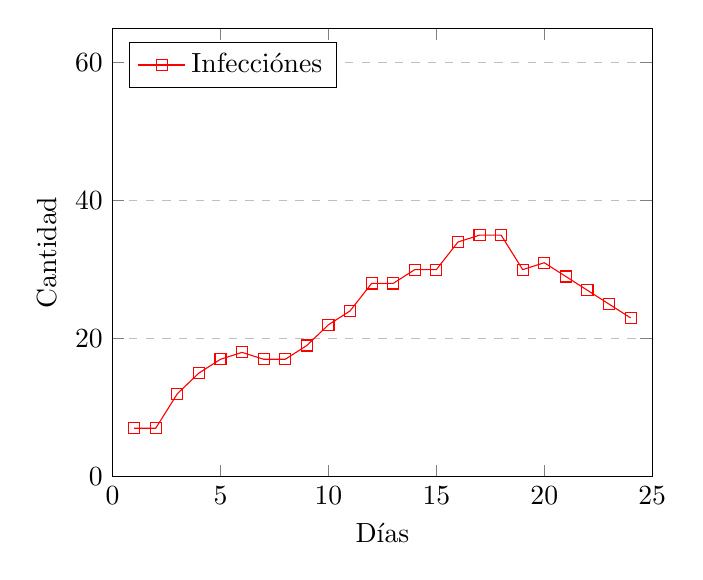
\begin{tikzpicture}
\begin{axis}[
xlabel={D\'ias},
ylabel={Cantidad},
xmin=0, xmax=25,
ymin=0, ymax=65,
legend pos=north west,
ymajorgrids=true,
grid style=dashed,
]
\addplot[
color=red,
mark=square,
]
coordinates {
(1, 7)(2, 7)(3, 12)(4, 15)(5, 17)(6, 18)(7, 17)(8, 17)(9, 19)(10, 22)(11, 24)(12, 28)(13, 28)(14, 30)(15, 30)(16, 34)(17, 35)(18, 35)(19, 30)(20, 31)(21, 29)(22, 27)(23, 25)(24, 23)
};
\legend{Infecci\'ones}
\end{axis}
\end{tikzpicture}
\newpage
\section{Cambios en el mapa}
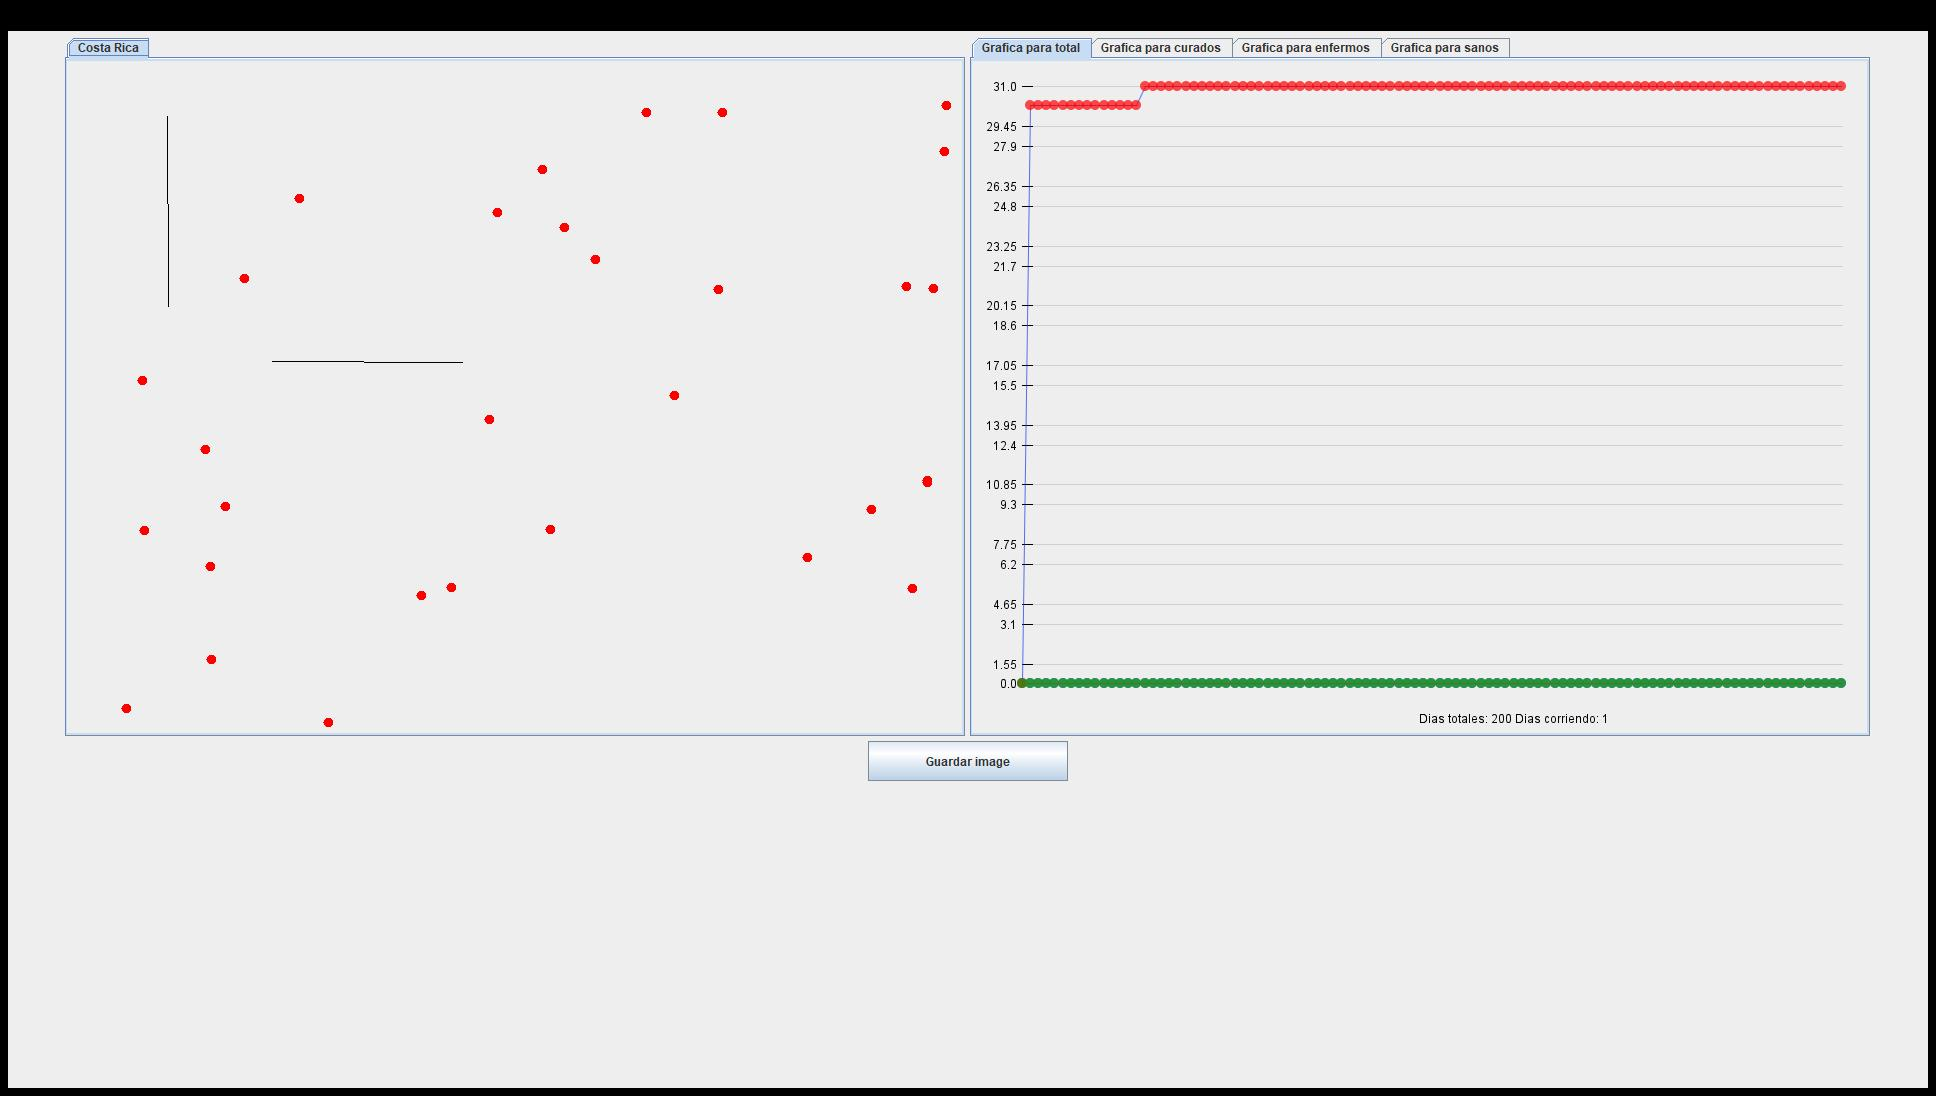
\includegraphics[scale=0.20]{1}
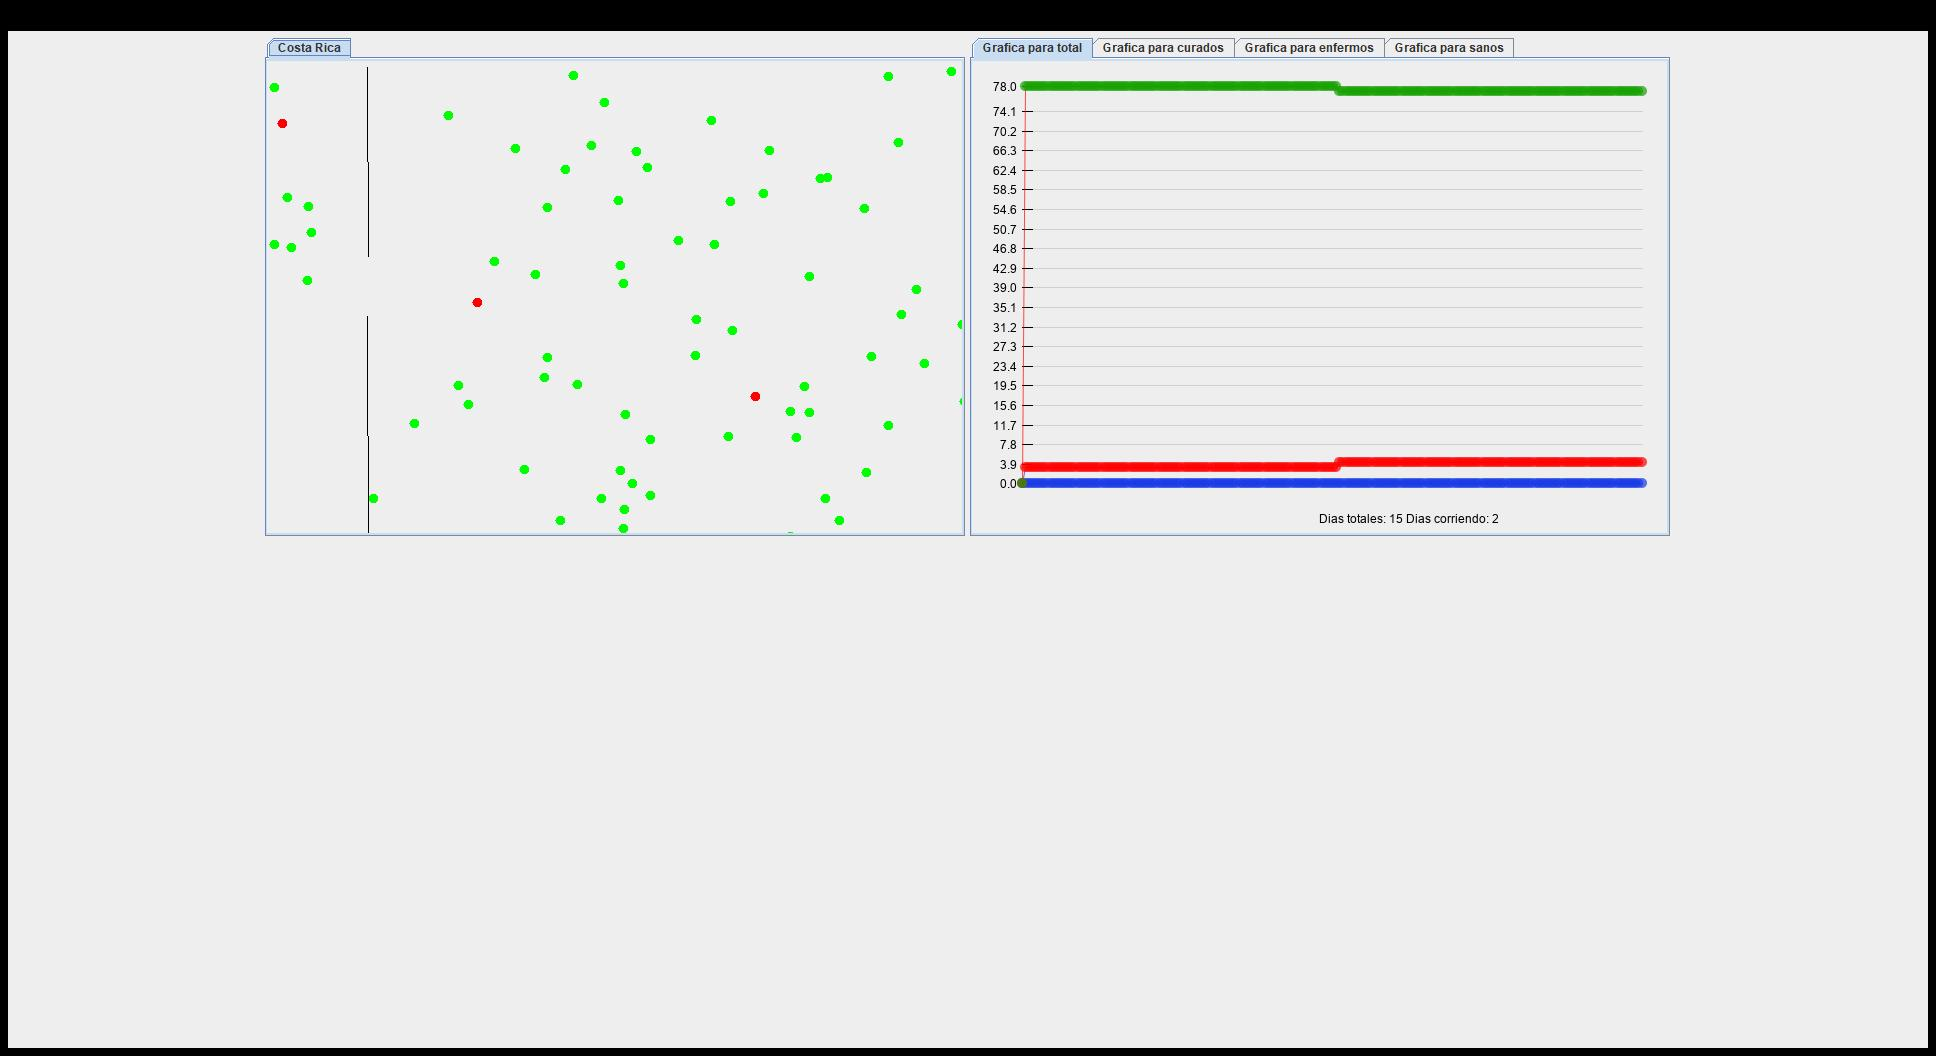
\includegraphics[scale=0.20]{2}
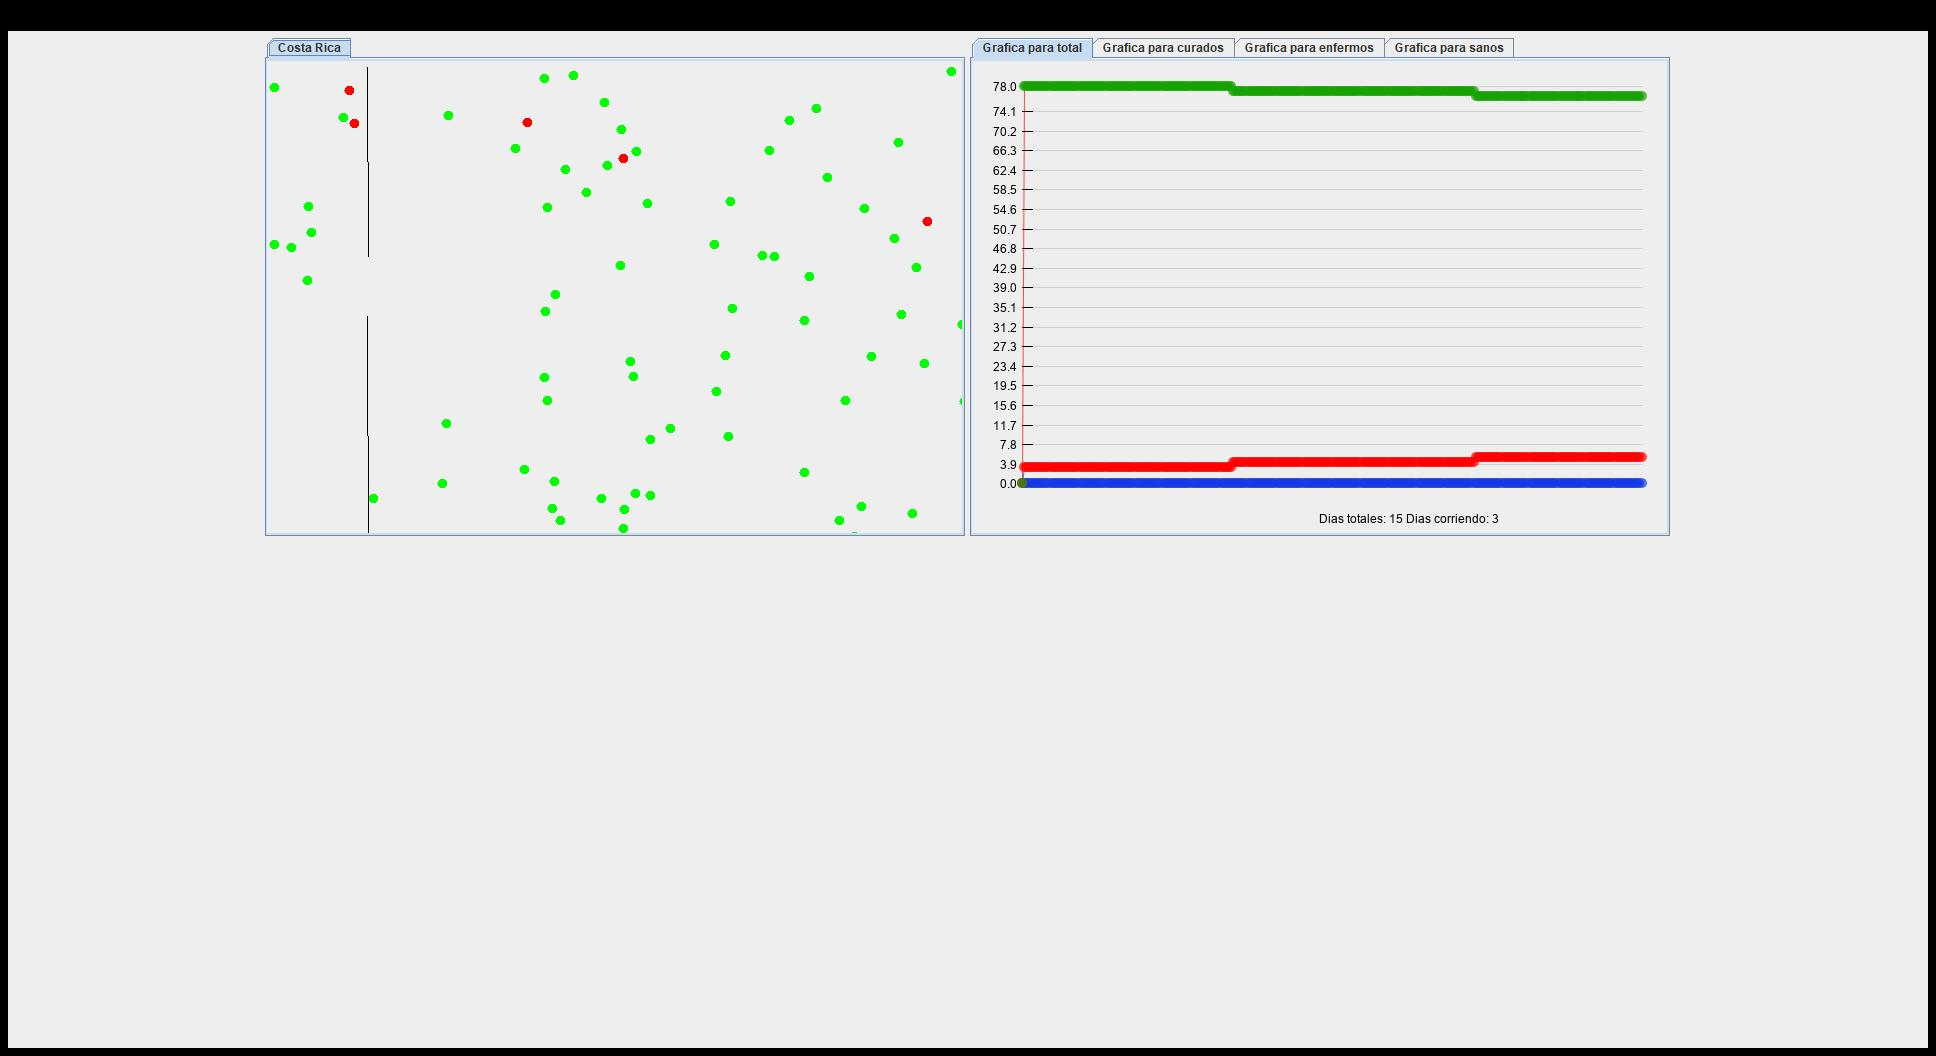
\includegraphics[scale=0.20]{3}
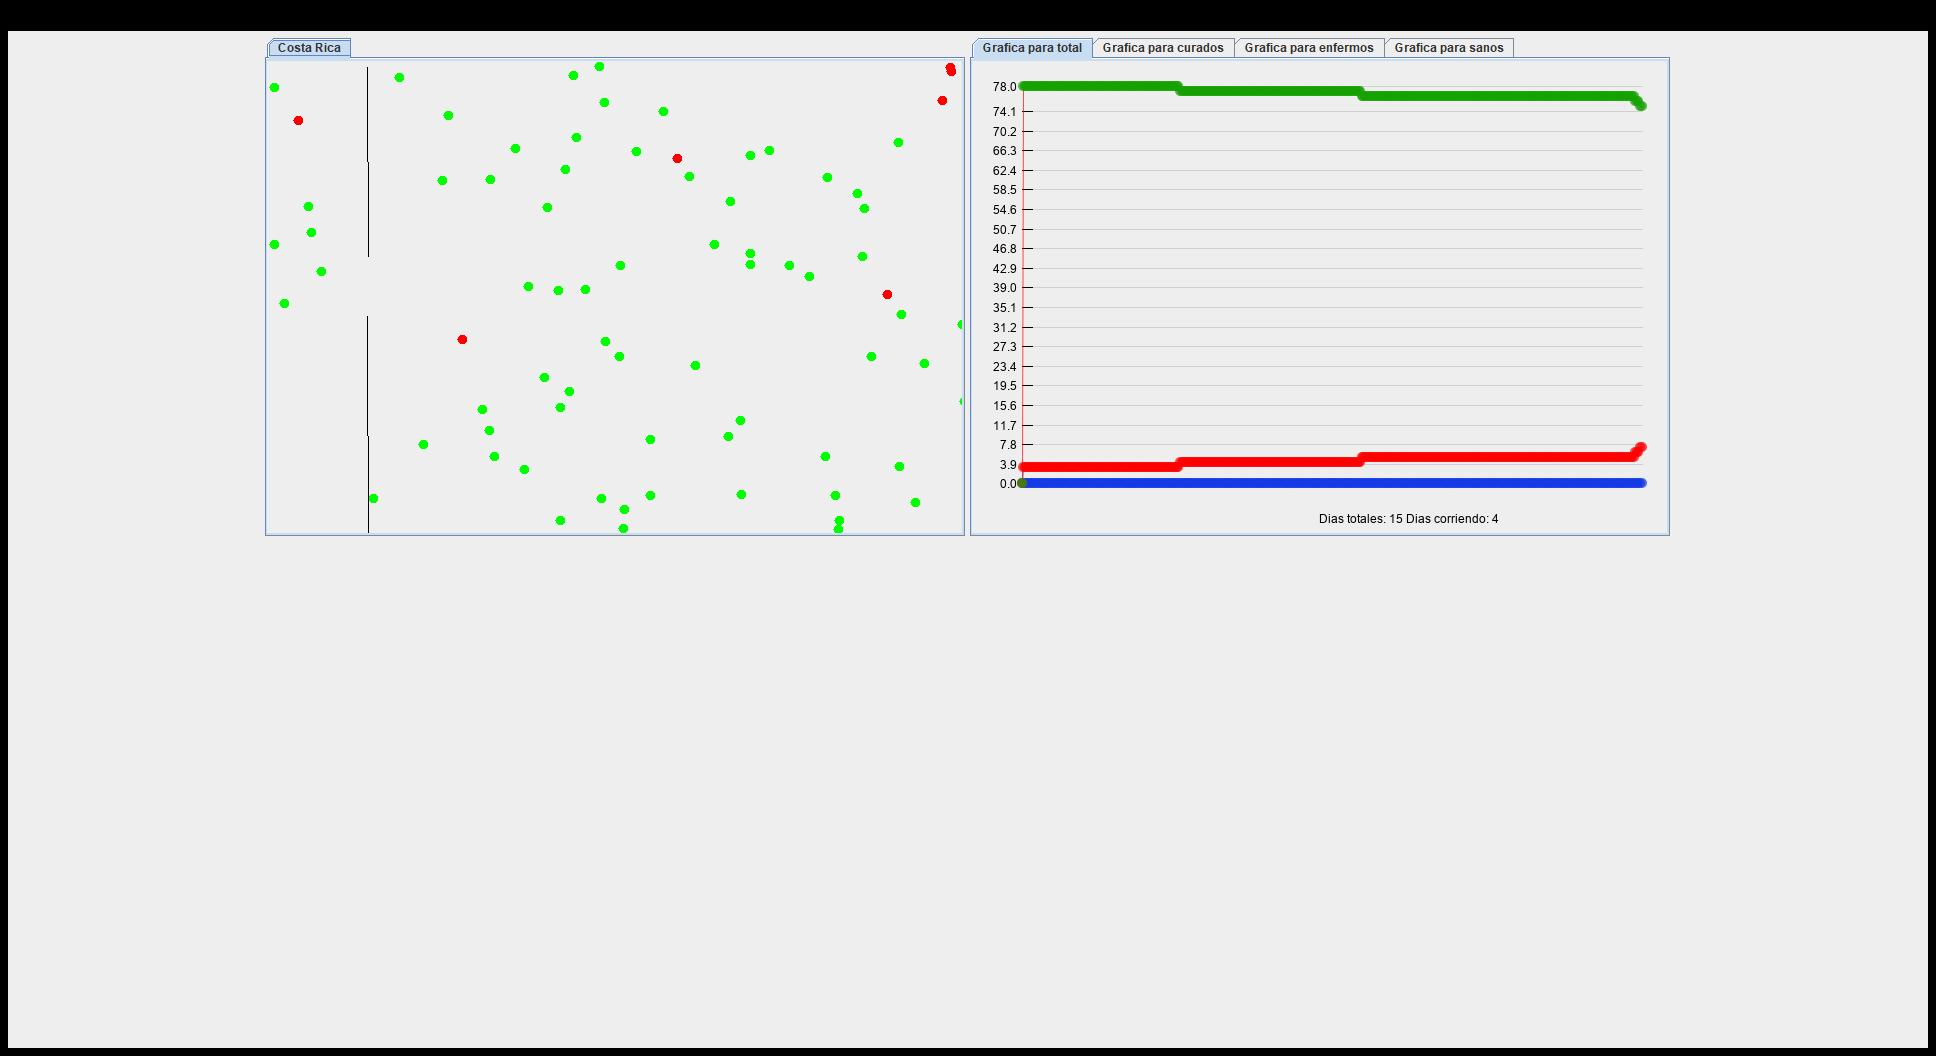
\includegraphics[scale=0.20]{4}
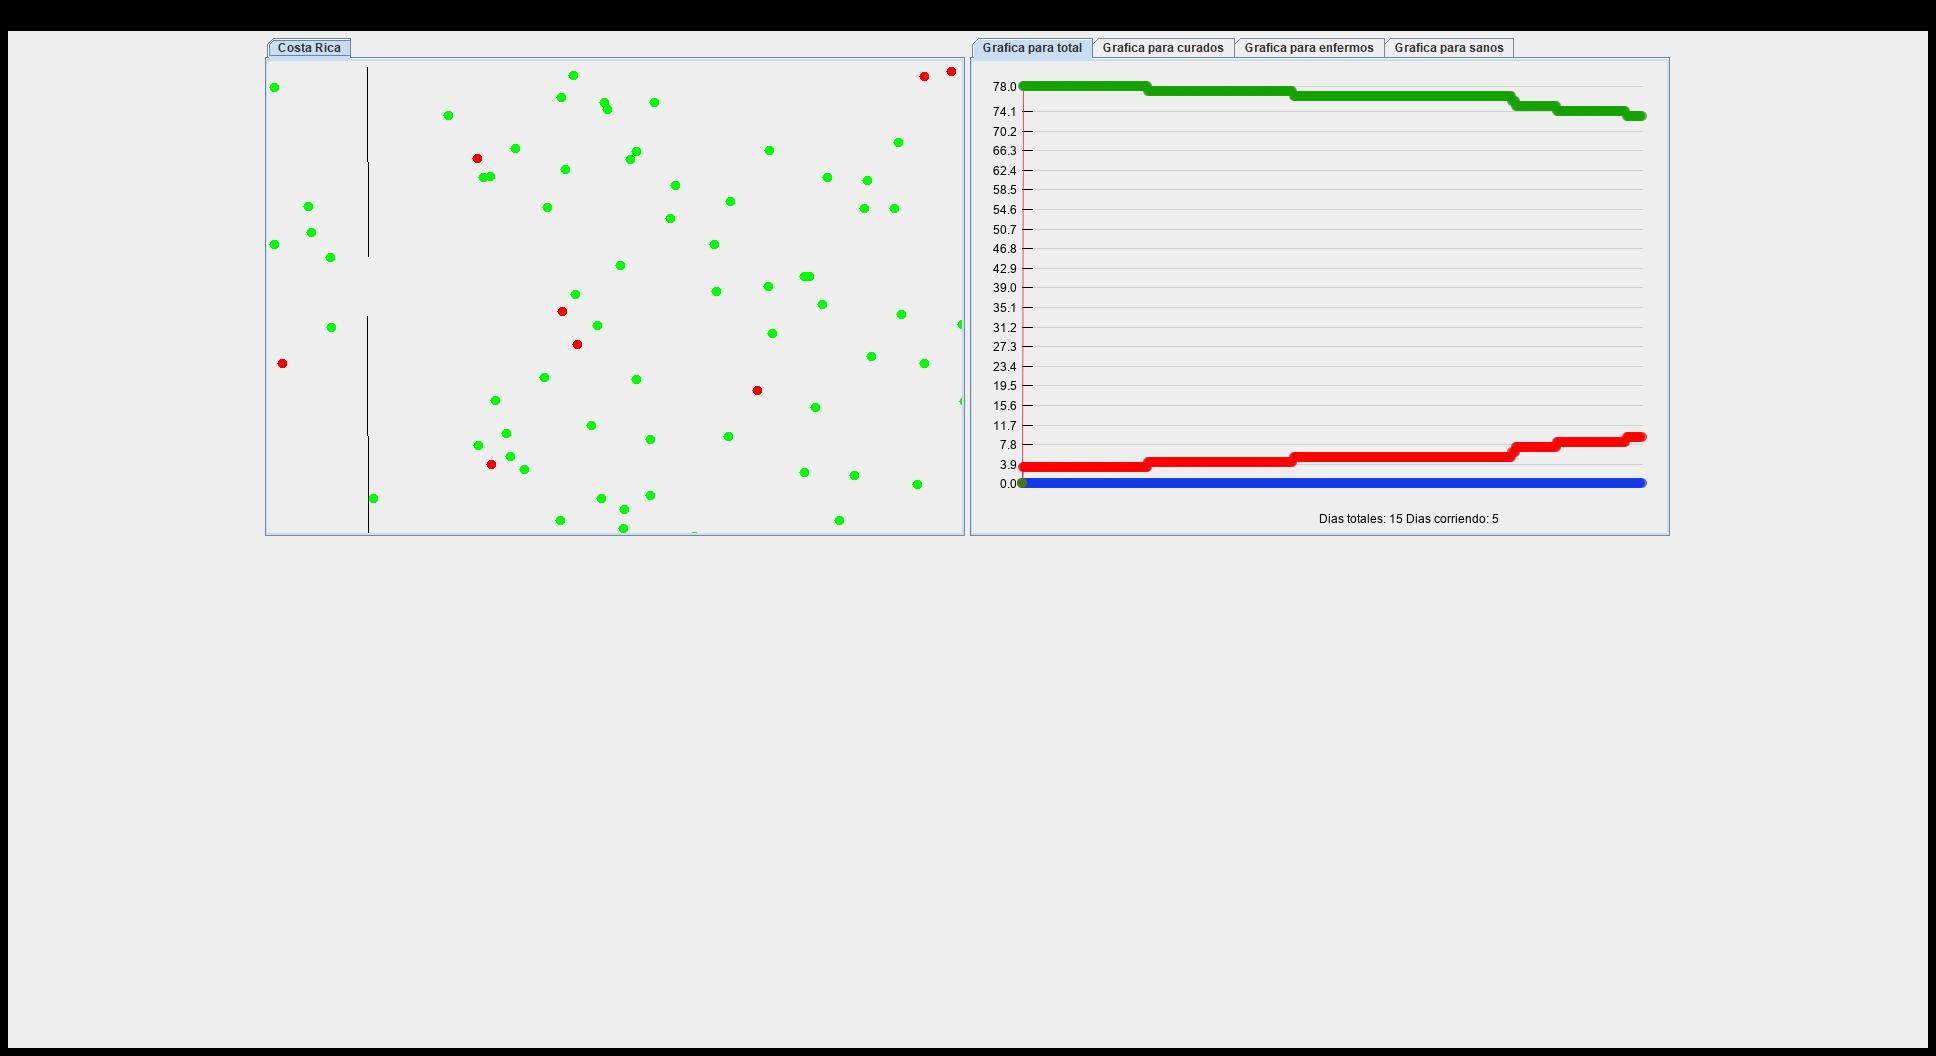
\includegraphics[scale=0.20]{5}
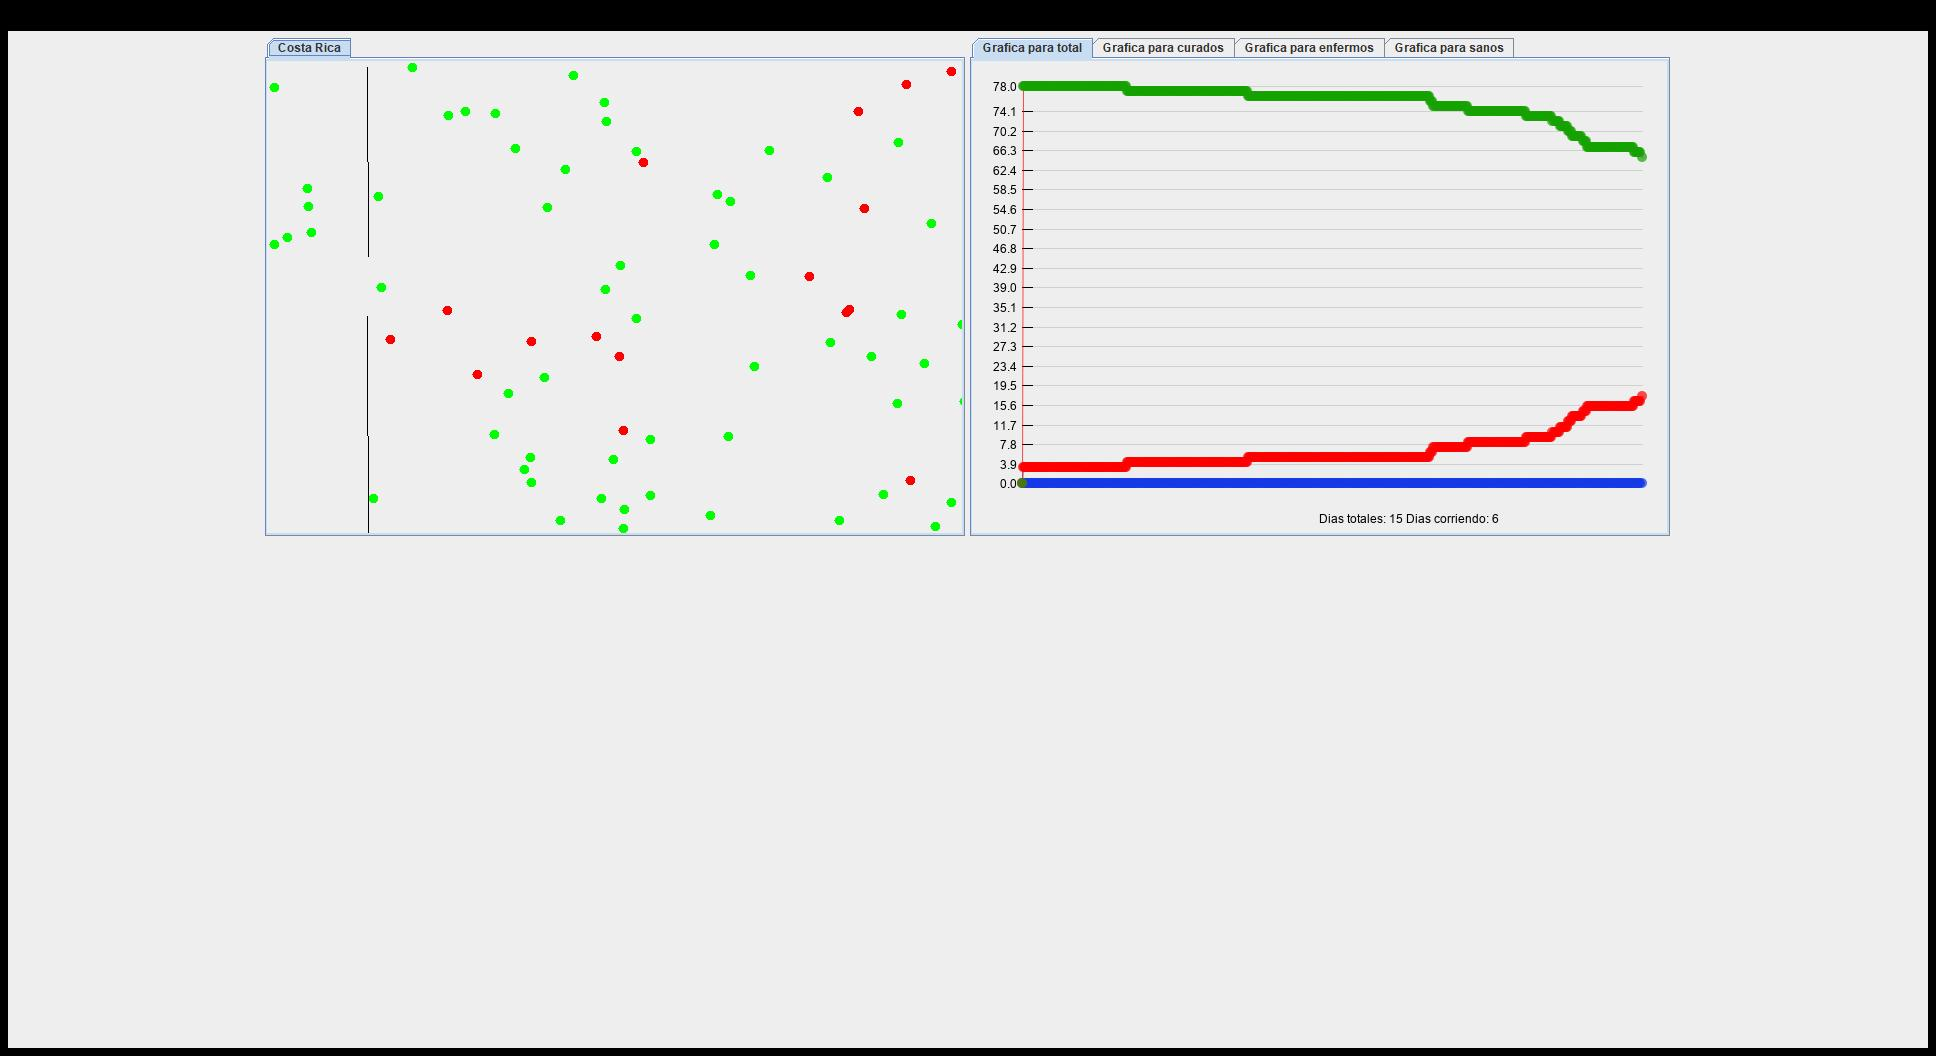
\includegraphics[scale=0.20]{6}
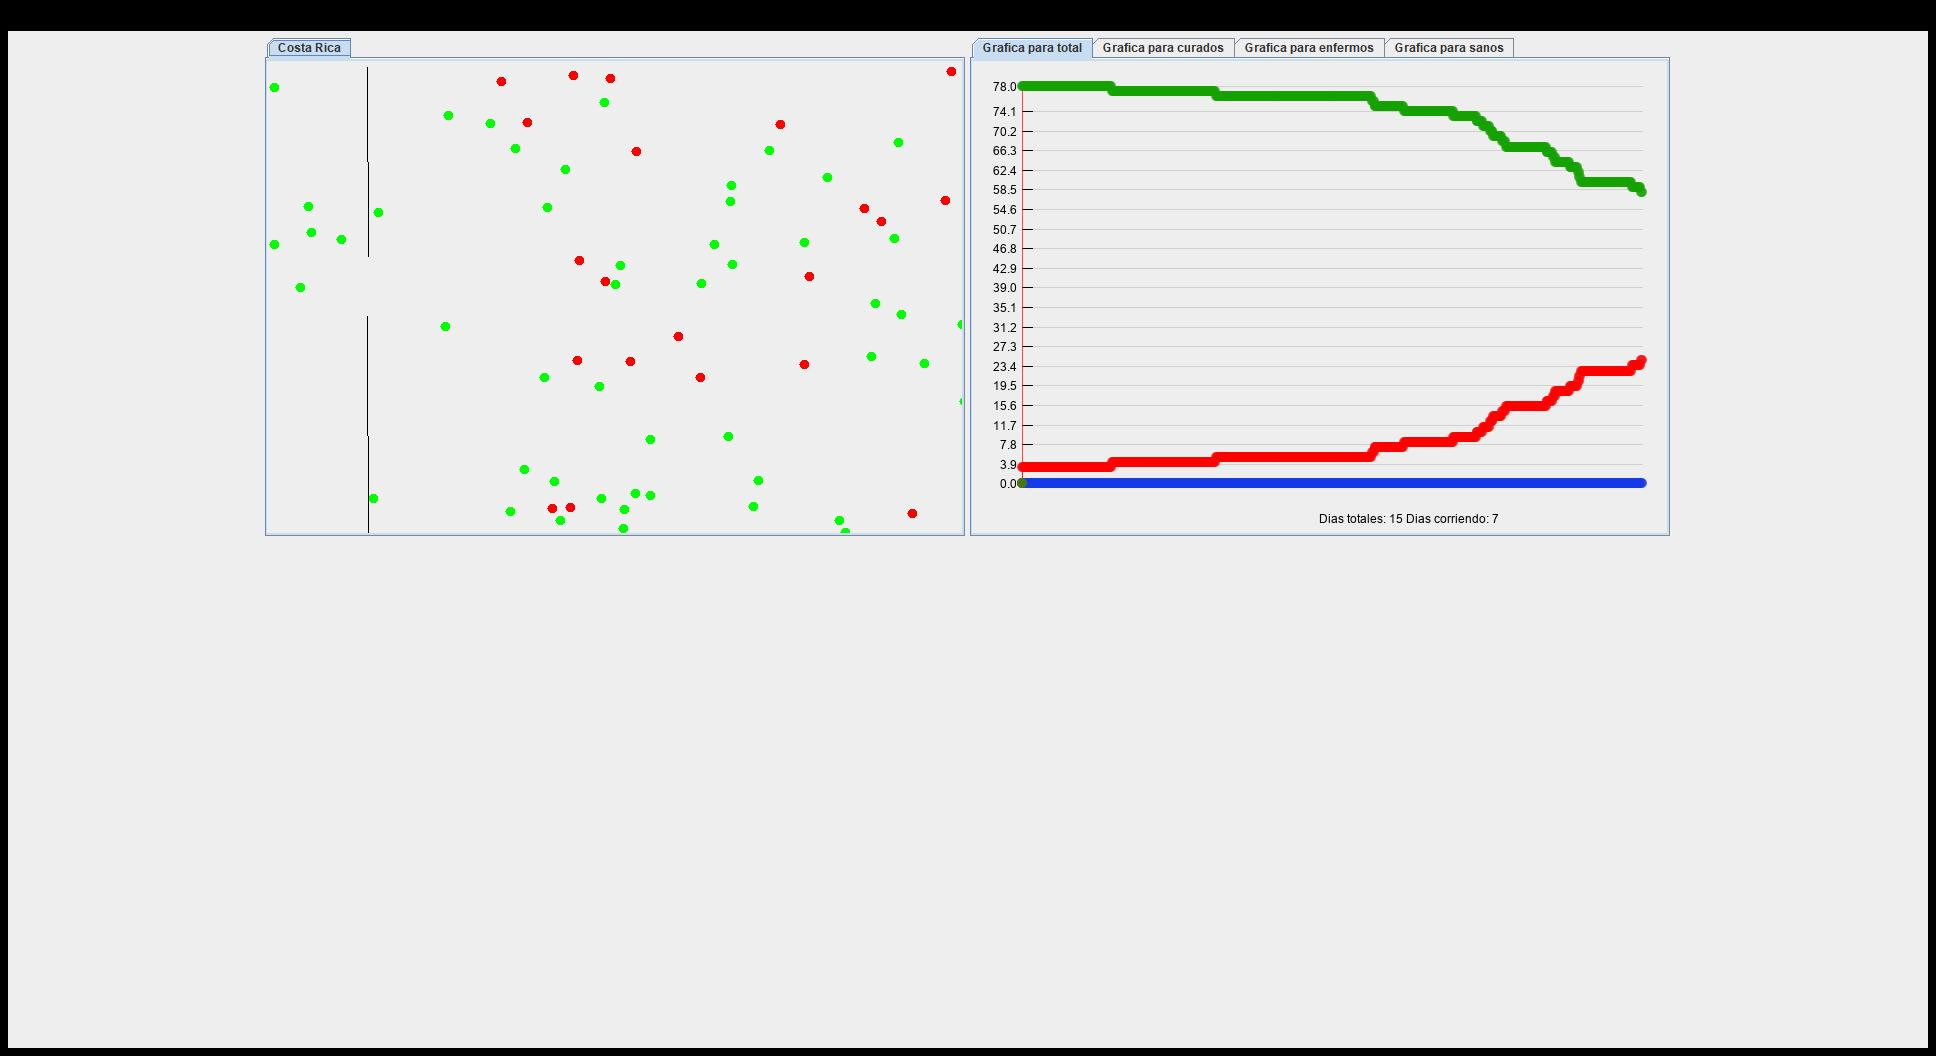
\includegraphics[scale=0.20]{7}
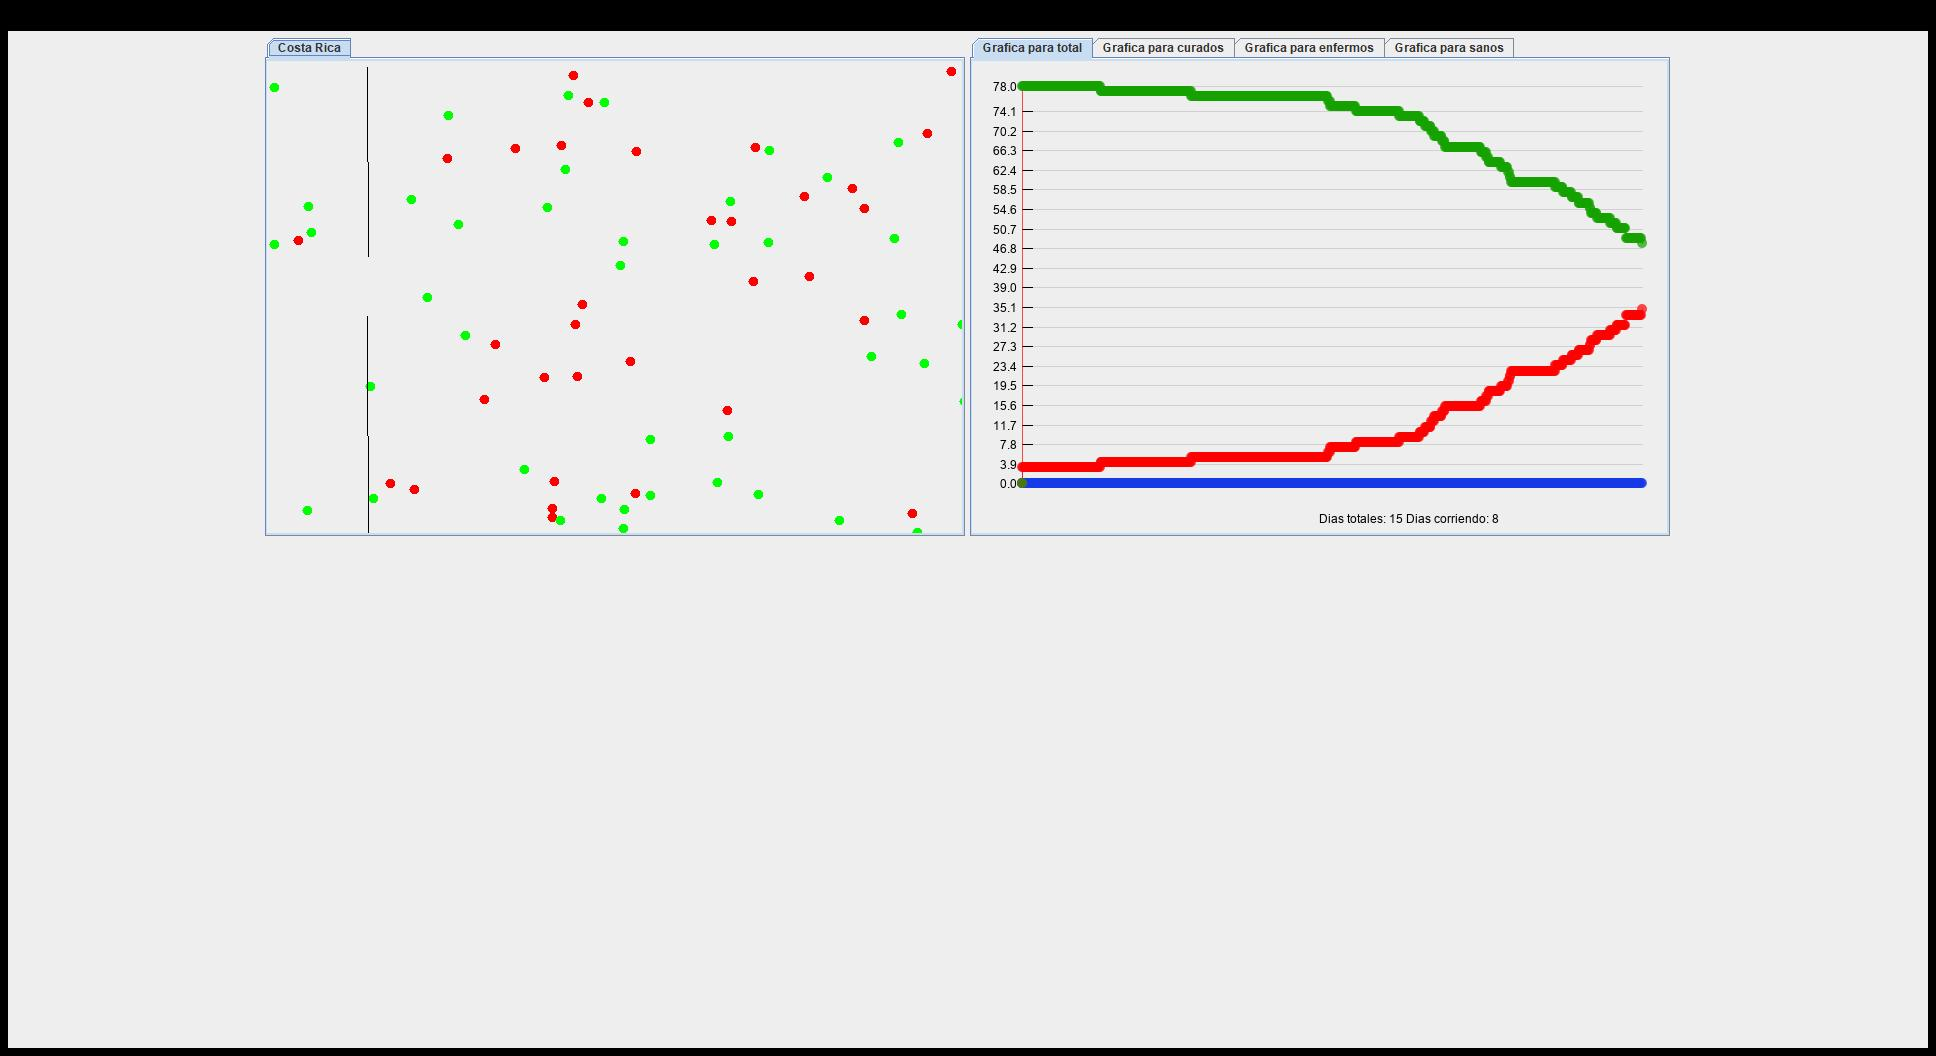
\includegraphics[scale=0.20]{8}
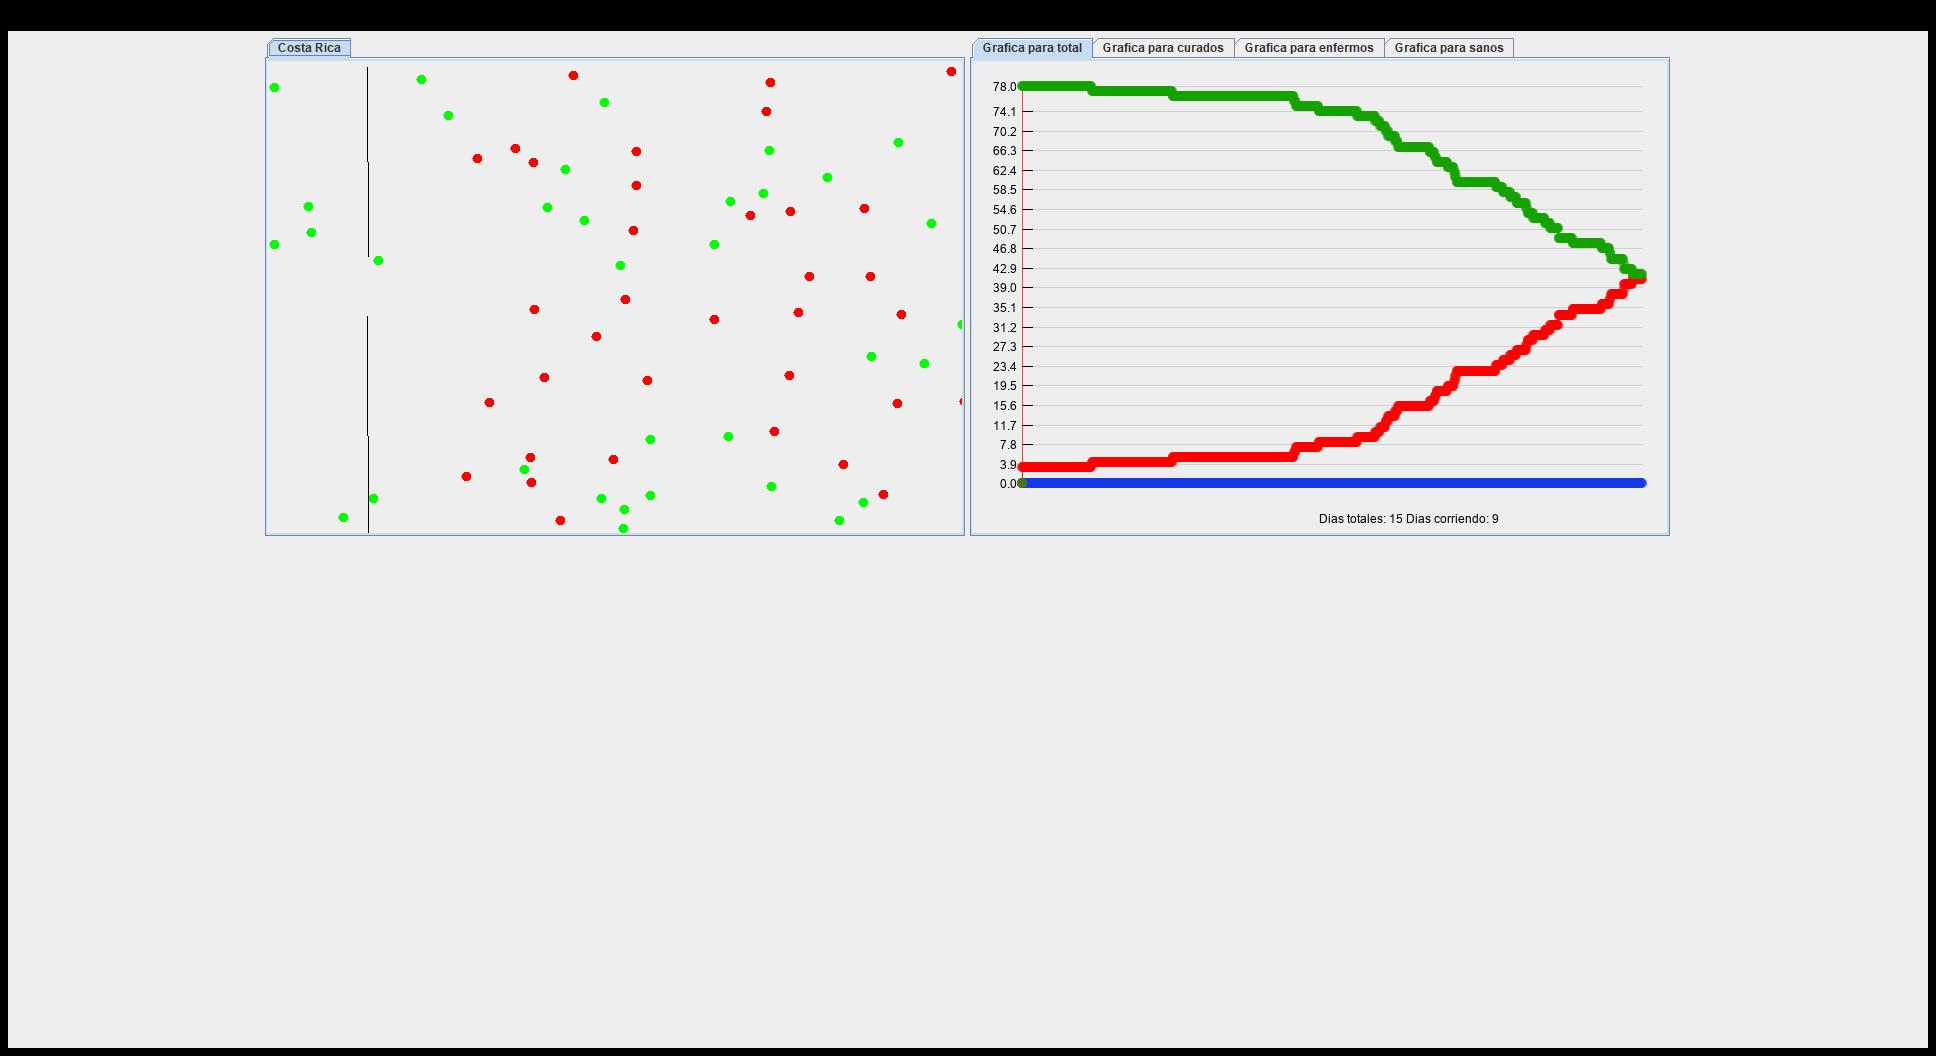
\includegraphics[scale=0.20]{9}
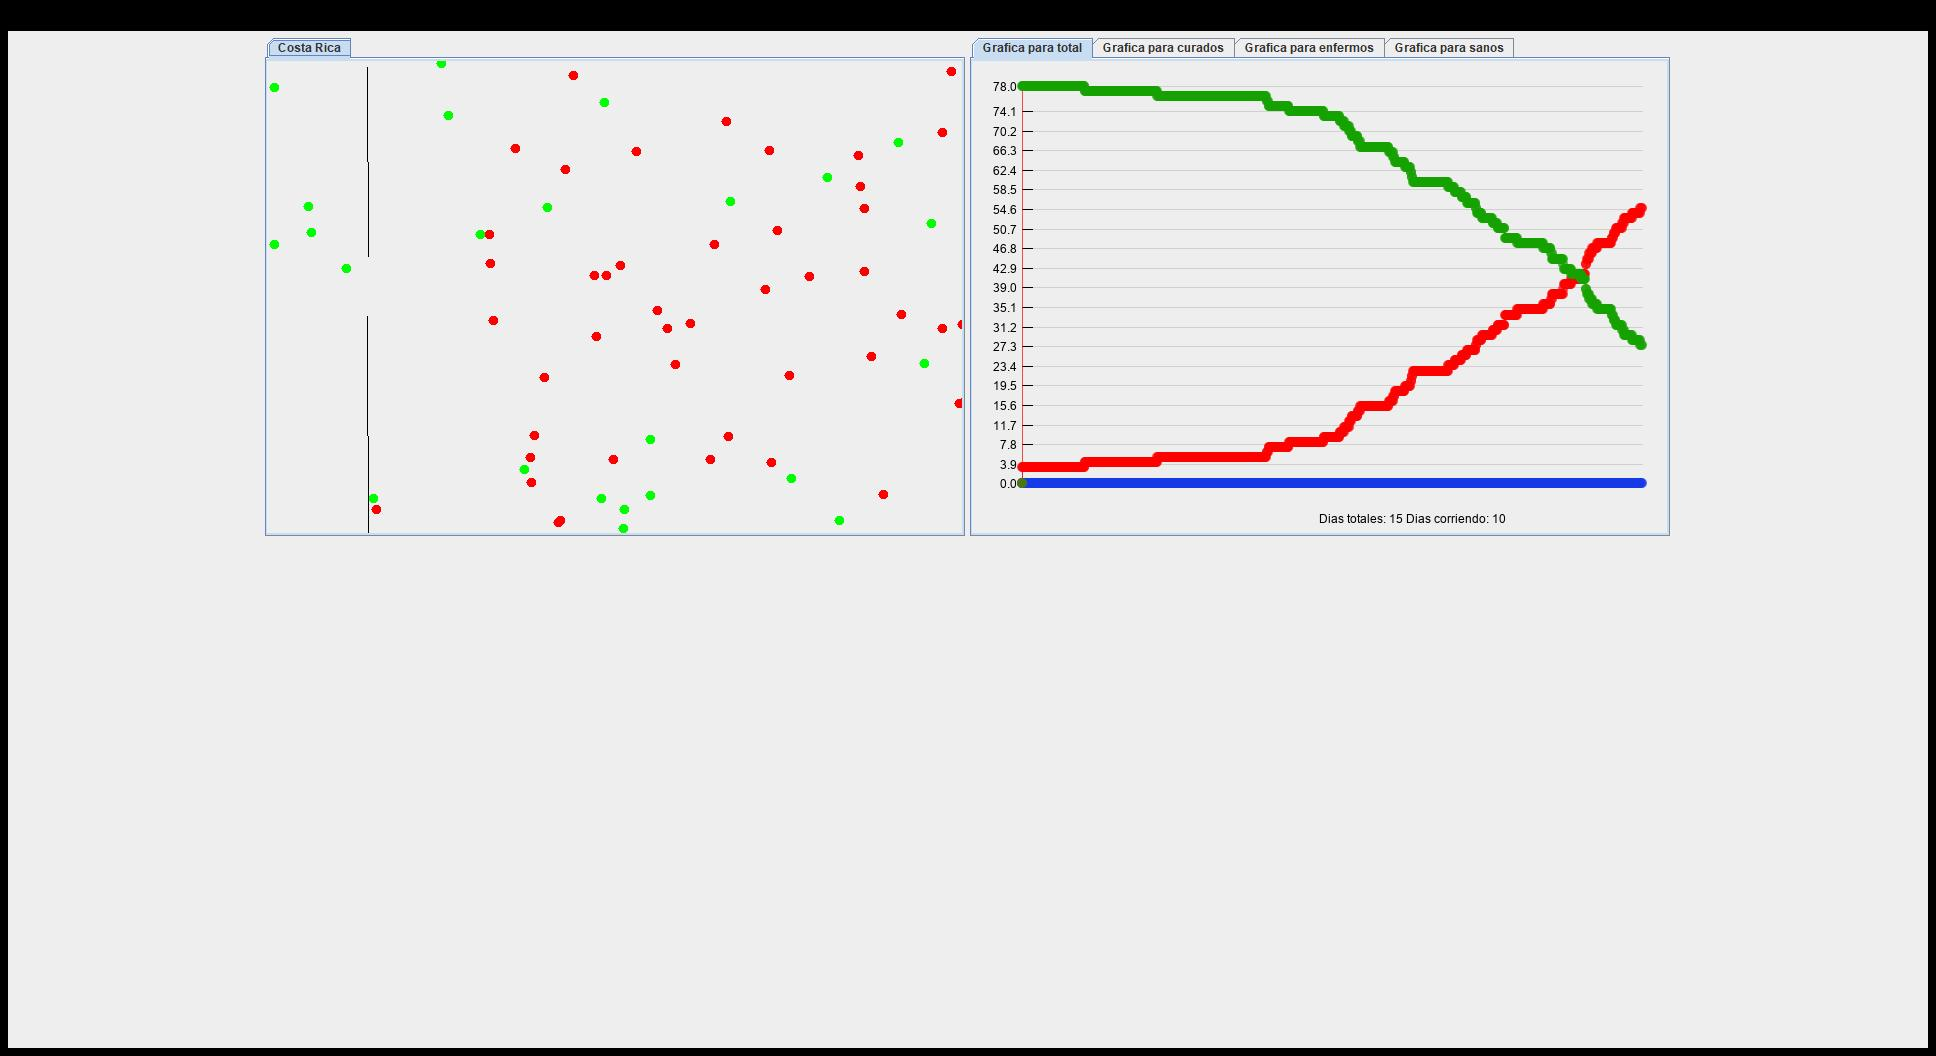
\includegraphics[scale=0.20]{10}
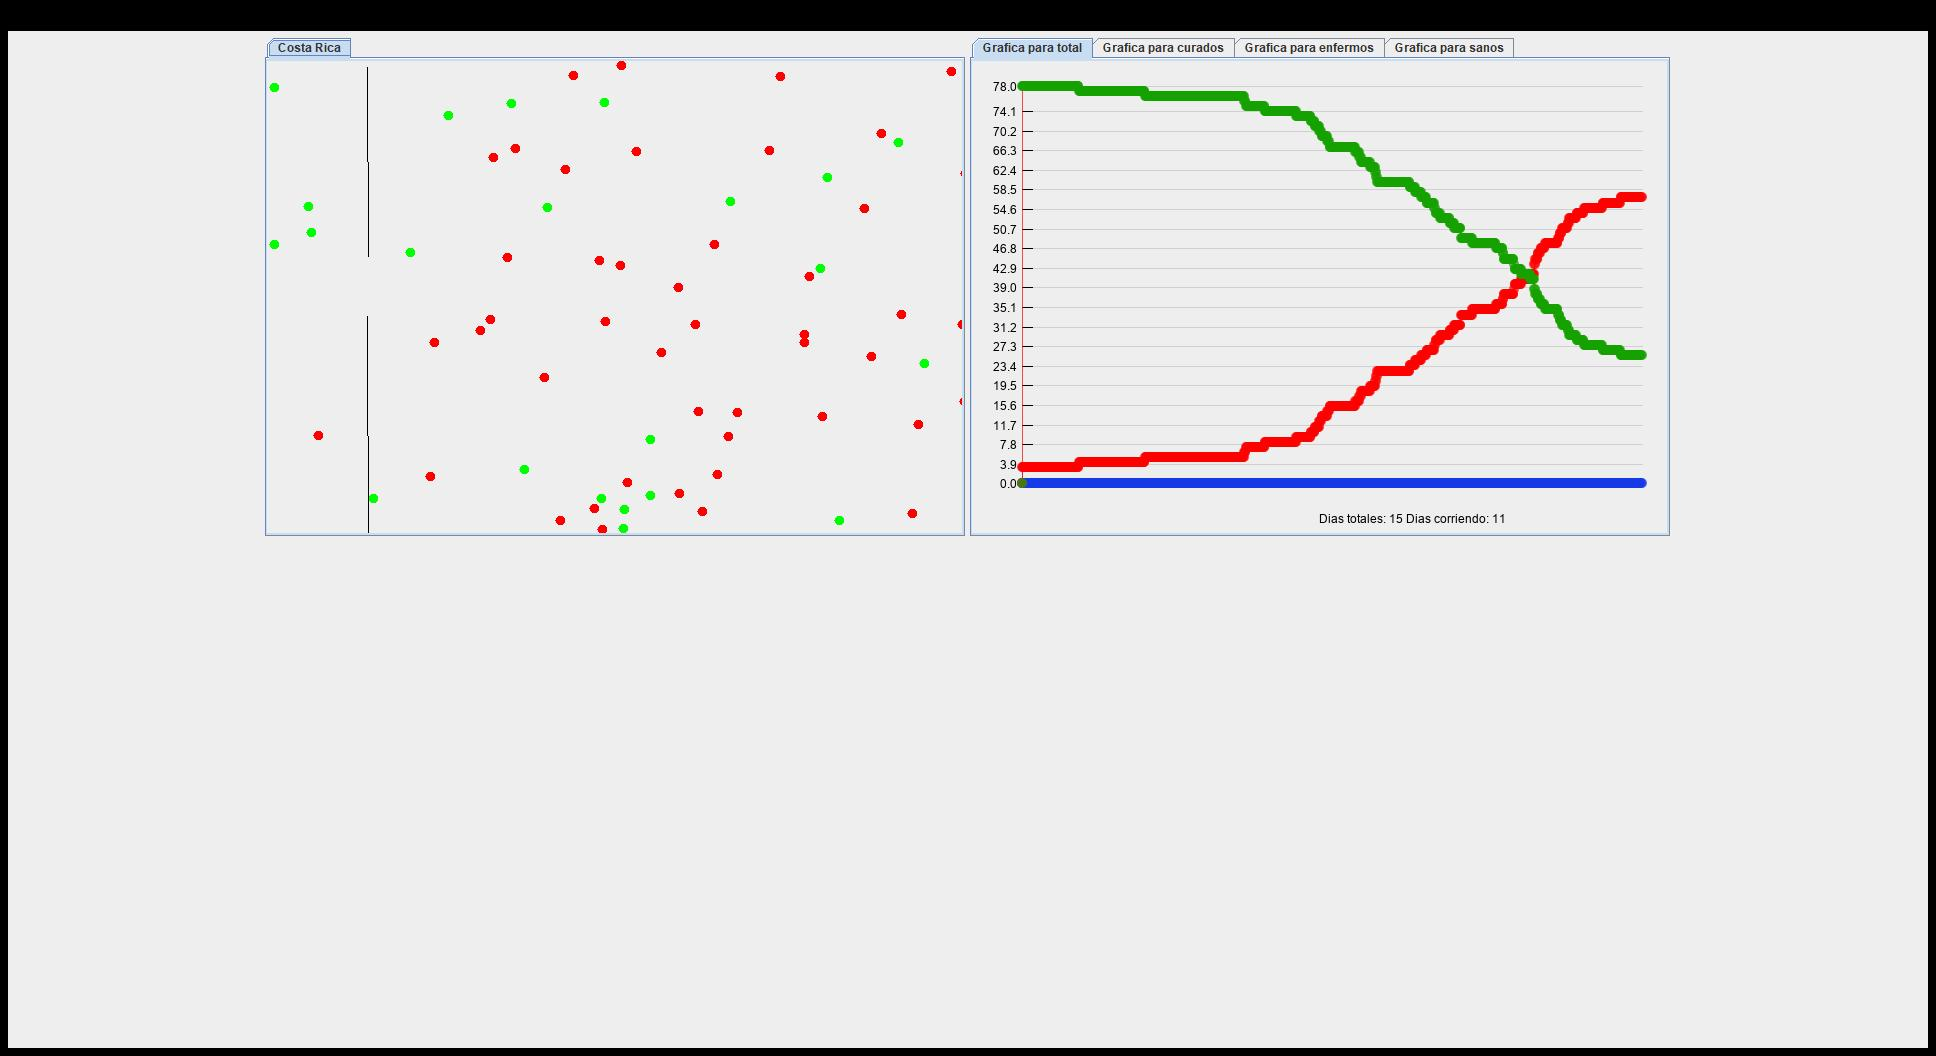
\includegraphics[scale=0.20]{11}
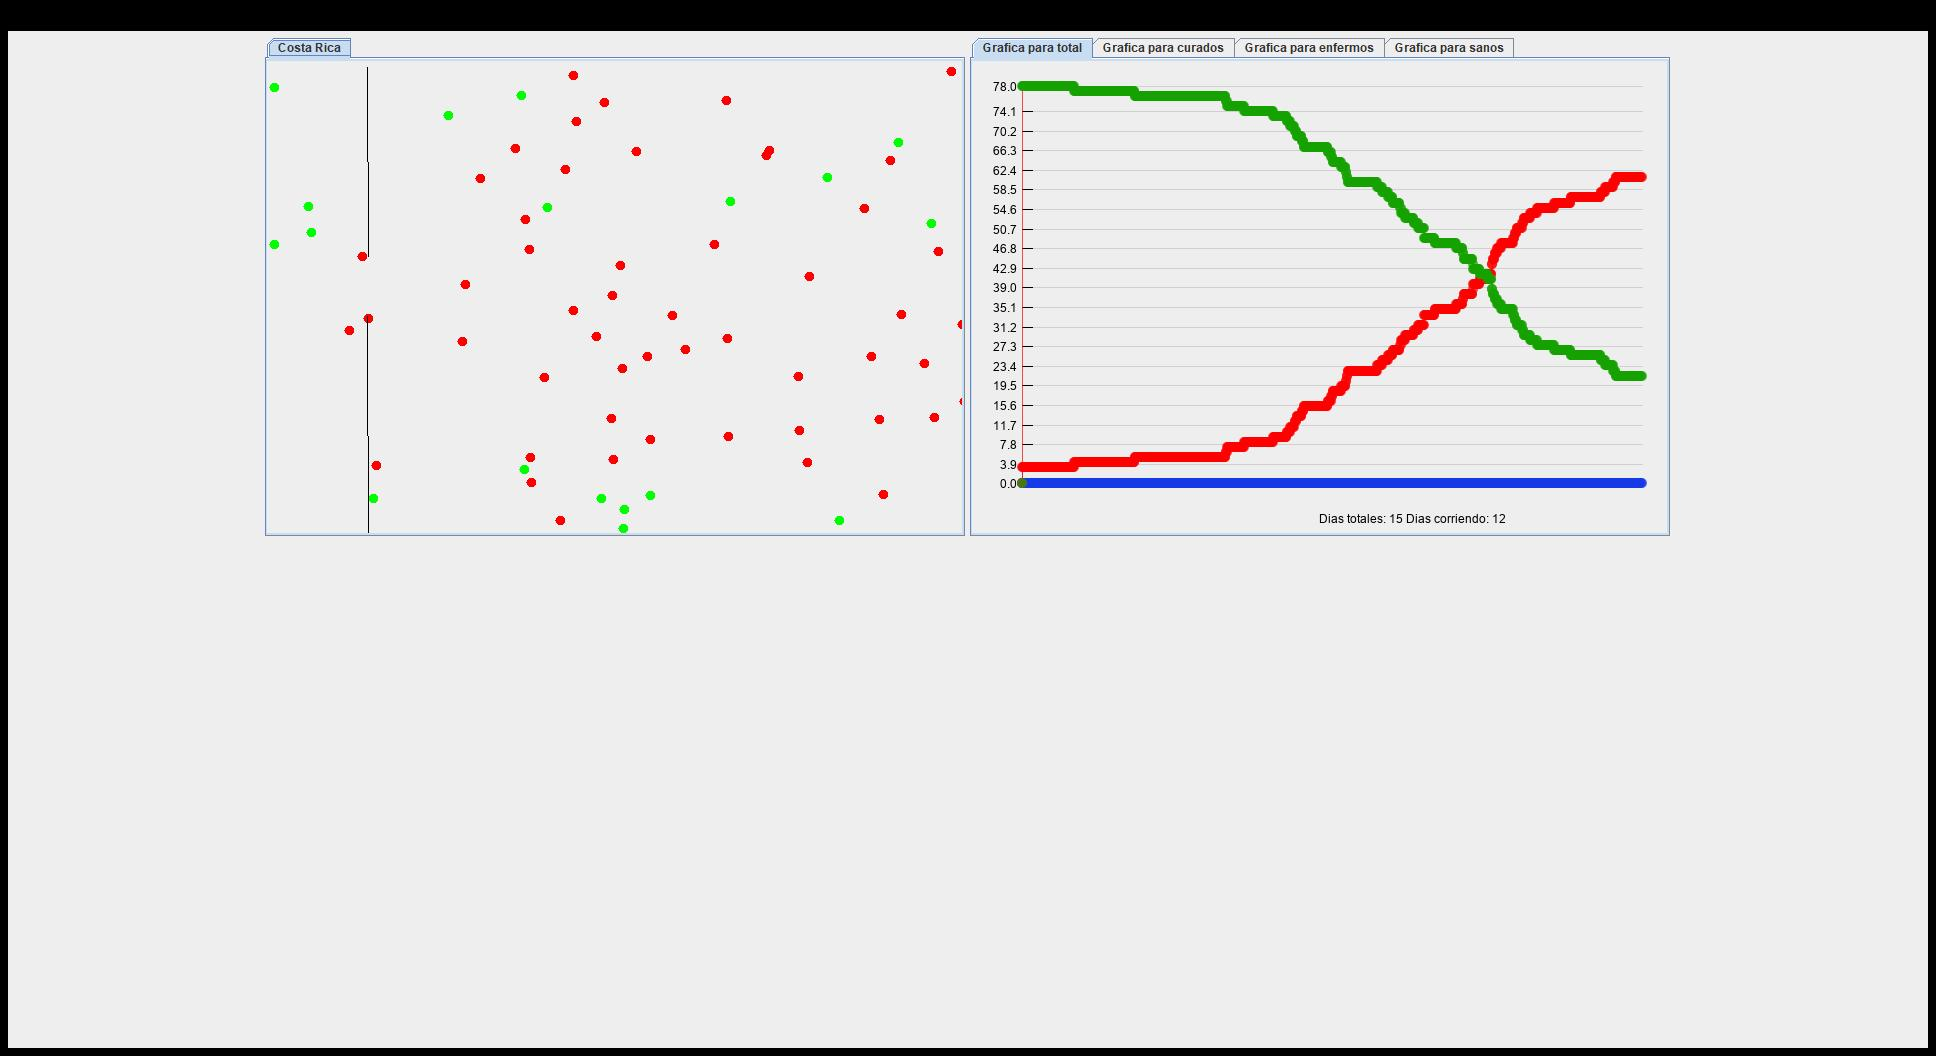
\includegraphics[scale=0.20]{12}
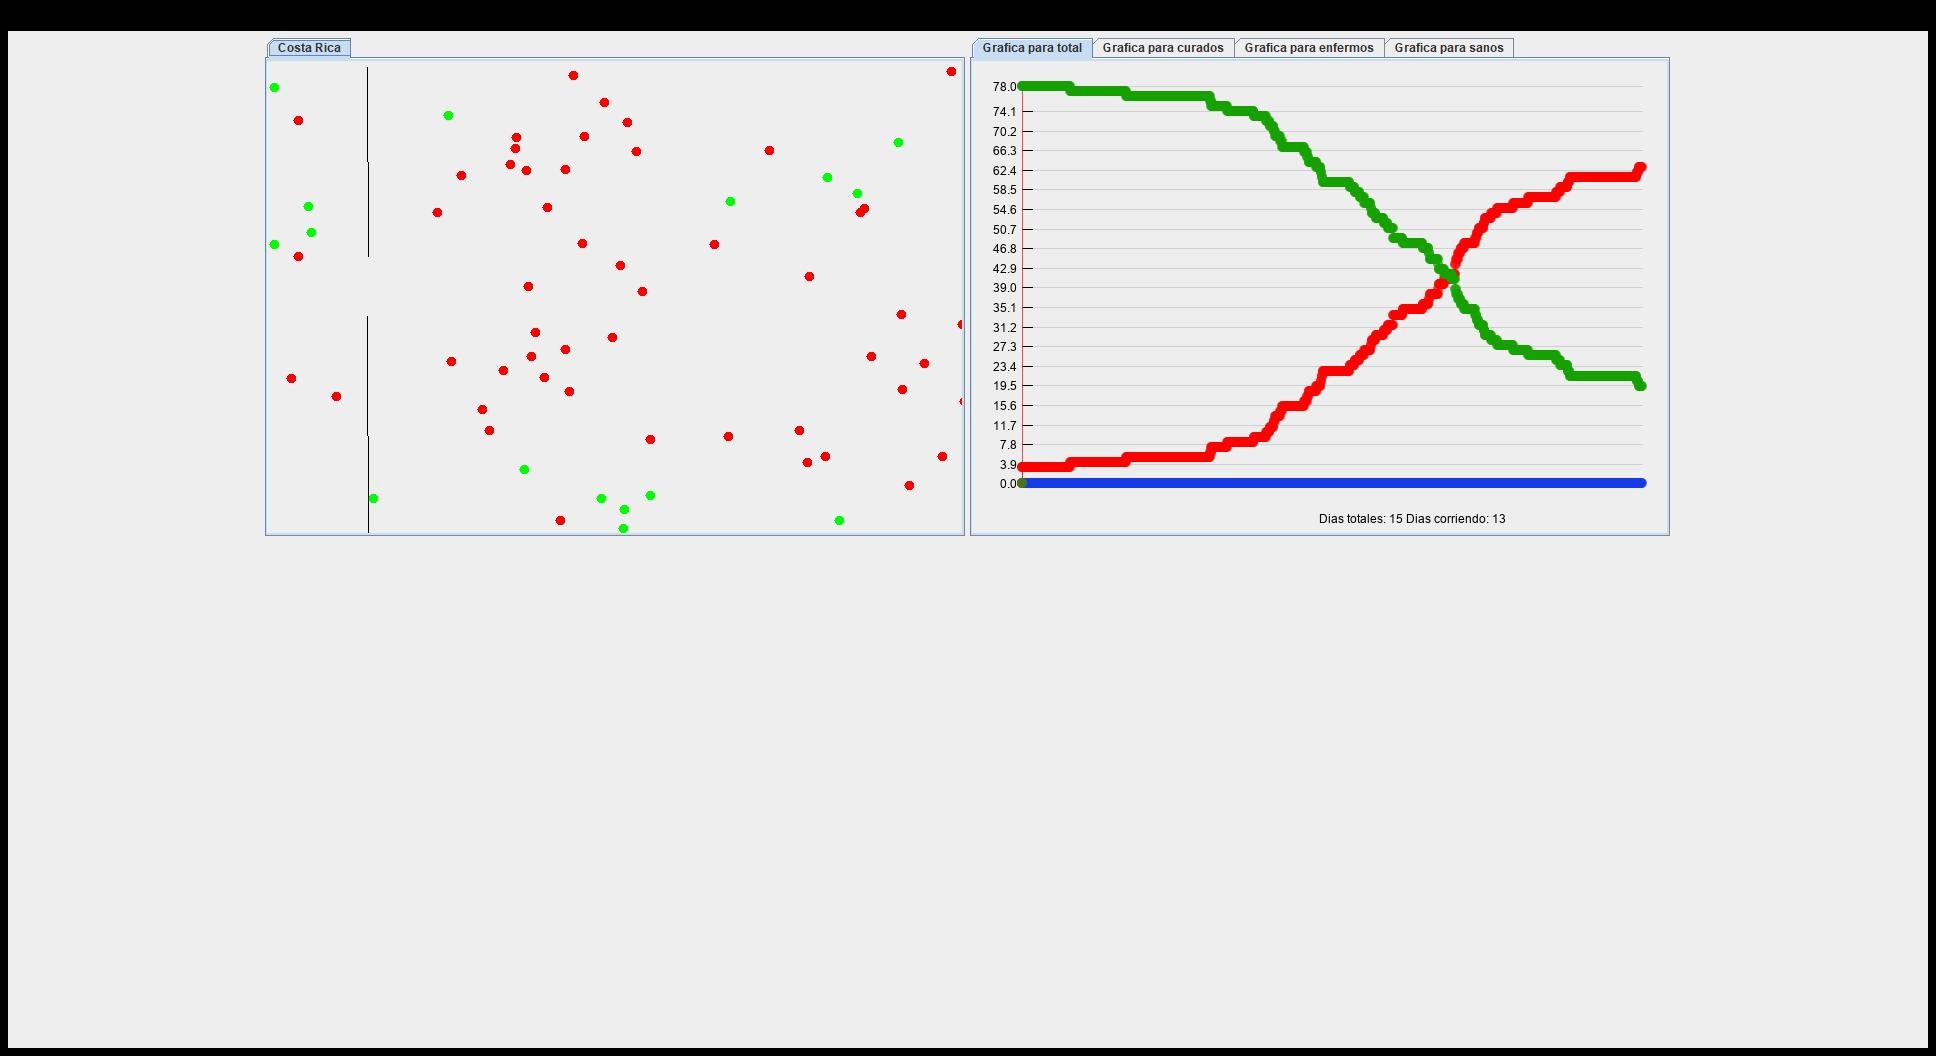
\includegraphics[scale=0.20]{13}
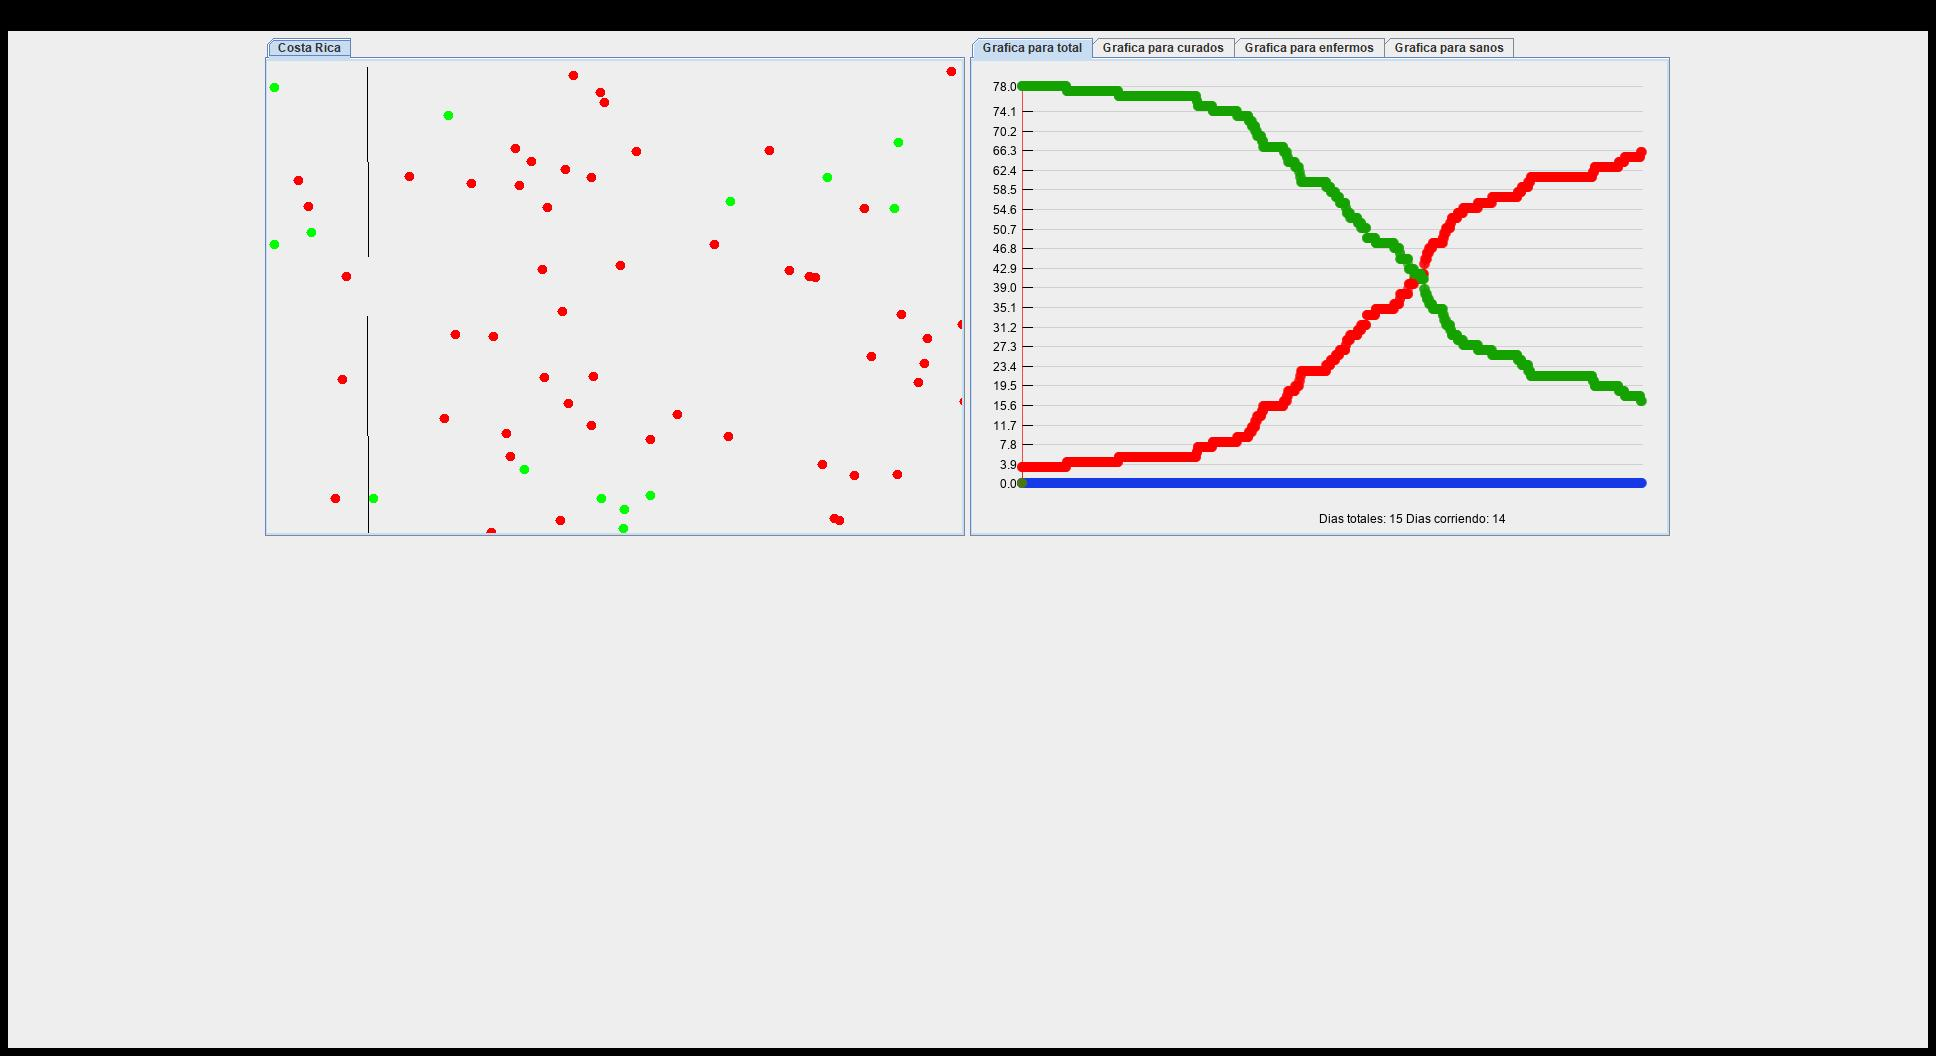
\includegraphics[scale=0.20]{14}
\includegraphics[scale=0.20]{15}
\includegraphics[scale=0.20]{16}
\includegraphics[scale=0.20]{17}
\includegraphics[scale=0.20]{18}
\includegraphics[scale=0.20]{19}
\includegraphics[scale=0.20]{20}
\newpage
\section{Viajes}
En el d\'ia 4 viajaron un total de 4 agentes.\n
En el d\'ia 5 viajaron un total de 5 agentes.\n
En el d\'ia 7 viajaron un total de 3 agentes.\n
En el d\'ia 9 viajaron un total de 1 agentes.\n
En el d\'ia 13 viajaron un total de 2 agentes.\n
En el d\'ia 15 viajaron un total de 2 agentes.\n
En el d\'ia 17 viajaron un total de 3 agentes.\newline
\end{document}
